\title{skycell: a cost-based HEALPix index for sky positions in PostgreSQL}
\subtitle{Design, brute-force validation, and a comparison with Q3C and pgSphere}

\author{J. Salgado\inst{1}}

%% Fill in before submission -- these are placeholders, not a real affiliation.
\institute{\textit{[affiliation]}\\
  \email{[e-mail address]}}

\date{Received ...; accepted ...}

\abstract
% context
{Astronomical archives answer positional queries from relational databases, and in the
PostgreSQL world two extensions dominate: Q3C, which keys each source by an integer
drawn from a quad-tree on a cube and stores it in a B-tree, and pgSphere, which stores
spherical geometry in a GiST tree. The first is compact and fast for points; the second
is general and indexes regions as well.}
% aims
{We ask whether the two can be combined: a single index that keeps the integer key and
the B-tree, yet answers cones, polygons, cross-matches and stored footprints, and that
speaks the geometry language archives already use.}
% methods
{We present \texttt{skycell}, a PostgreSQL extension that keys positions by their
order-29 HEALPix cell in the nested scheme and turns any query region into a small set
of index ranges. How finely to cut is decided by a cost model -- the price of an extra
index range against the rows it removes -- with the local source density read from the
histogram \texttt{ANALYZE} already keeps for the key column, which is a density map
precisely because HEALPix cells are equal area. Cells are classified against the region
by their own corner geometry, the cell order follows in closed form, and a planner
support function rewrites the predicate into B-tree range conditions plus an exact test
before path generation. Correctness is established by brute force: coverings are checked
against millions of catalogue points and against points sampled inside adversarial
cones. Performance is measured on a 10-million-source synthetic catalogue with
Gaia-like crowding, against Q3C 2.0.5 and pgSphere 1.5.2 on identical data, and in an
A/B test inside a working TAP service.}
% results
{On the synthetic catalogue the median cone search is faster than both extensions at
every radius tested, from 1\arcsec\ to 3\degr\ (for example 0.024\,ms against
0.035\,ms for pgSphere and 1.330\,ms for Q3C at 1\arcsec, and 0.573\,ms against
1.010\,ms and 3.023\,ms at 3\degr), while touching about half of pgSphere's buffer
pages at large radii and keeping an index of 214\,MB against pgSphere's 683\,MB.
Convex polygons are four times faster than pgSphere's, a 200\,000-probe cross-match at
1\arcsec\ takes 0.47\,s against 1.95\,s for Q3C and 2.85\,s for pgSphere, and the
planner's row estimates are 1.2 times off instead of 1.9--2.8. A control measurement
that interleaves the two methods query by query, with skycell measured first, reduces
the cone-search advantage to a factor 0.61--1.04. On a 500\,096-row ObsCore table
inside a TAP server the same build is 1.2--1.45 times \emph{slower} per query than
pgSphere, and all 18 end-to-end comparison cells tie.}
% conclusions
{A cost-based covering over an equal-area integer key is competitive with both
established designs on large catalogues and keeps the generality of a geometry type,
at the price of planning work that only pays off once the scan dominates the query.
The crossover in these measurements is a few million rows.}

\keywords{Astronomical databases: miscellaneous -- Catalogs -- Virtual observatory tools --
  Methods: data analysis}

\maketitle

\section{Introduction}

Almost every question asked of an astronomical archive is positional: what is within
this cone, which observations cover this field, which of my sources match that
catalogue. In the Virtual Observatory these questions arrive as ADQL
\citep{adql} through the Table Access Protocol \citep{tap}, and the service has to turn
them into something a relational database can answer with an index.

Two PostgreSQL extensions carry most of this traffic. Q3C \citep{q3c} projects the
sphere onto a cube, subdivides each face with a quad-tree, and numbers the cells along
a space-filling curve; each source is one 64-bit integer in a B-tree, and the table can
be sorted along the same curve so that neighbours on the sky are neighbours on disk.
pgSphere \citep{pgsphere} takes the other route: it adds spherical types -- points,
circles, polygons, boxes -- and indexes them with GiST over bounding volumes, so that
regions can be stored and queried as data, not only as query arguments.

Neither idea is new to astronomy. The Hierarchical Triangular Mesh \citep{htm} had
already keyed positions by a subdivided polyhedron, and the zones algorithm
\citep{zones} showed how far a purely relational arrangement -- declination strips and
a B-tree -- can be pushed for cross-matching. What has changed since is the size of the
catalogues and the fact that most queries now arrive through a generated layer
\citep[e.g.][]{dachs} rather than being written by hand, so the index has to serve a
translator's output rather than a tuned query.

The two designs trade off against each other. A linear key in a B-tree is compact,
cheap to probe and orders the heap, but a region has to be turned into a set of key
ranges before the index can be used, and a set of ranges is an approximation whose
quality depends on how finely the region is cut. A tree of bounding volumes has no such
approximation step and handles extended objects naturally, but its keys are larger, its
nodes overlap, and it imposes no useful order on the table.

This paper presents \texttt{skycell}, which keeps the integer key and asks a cost
question at the point where the classical approach fixes a constant: how finely should
a region be cut? The answer depends on two quantities the database already knows -- how
many sources sit in that part of the sky, and how much an extra index range costs --
and it can be computed rather than configured. Section~\ref{sec:method} develops the
method, Sect.~\ref{sec:impl} describes what it takes to make a query planner use it,
Sect.~\ref{sec:validation} the brute-force validation, Sects.~\ref{sec:bench}
and~\ref{sec:results} the measurements against Q3C and pgSphere, and Sect.~\ref{sec:tap}
an A/B test inside a working TAP service, which is where the method's limits show.

\section{Method}
\label{sec:method}

\subsection{An equal-area integer key}

A position is keyed by the HEALPix cell containing it at order 29 in the nested scheme
\citep{healpix}, a 64-bit integer addressing cells of about 0.4\,mas. Three properties
of that choice matter, and only the first is shared with the cube quad-tree of Q3C.

Cells are \emph{nested}: the descendants of a cell at any order form one contiguous
interval of order-29 ids, so a region covered by cells becomes a union of integer
ranges, and a B-tree can answer it.

Cells are \emph{equal area}. Every cell subtends the same solid angle, so the count of
keys in an interval divided by the interval's length is proportional to a source
density per unit area. The histogram that \texttt{ANALYZE} keeps for the key column is
therefore a map of how crowded each part of the sky is, at the resolution of its
buckets, without any extra statistics machinery.

Cells are \emph{standard}. The same numbering underlies Gaia's \texttt{source\_id}
\citep{gaia} and the IVOA's Multi-Order Coverage maps \citep{moc}, so keys, coverings
and stored footprints are interoperable rather than private to one extension.

\subsection{Coverings decided by cost}
\label{sec:cost}

A query region is covered by cells whose union contains it; the covering becomes range
conditions on the key, and rows inside the covering but outside the region are removed
by an exact test. Cutting finer means fewer such false positives and more ranges. With
cells of size $s$ covering a region of characteristic radius $r$ and a local source
density $\rho$ (sources per unit solid angle),

\begin{equation}
  C(s) = n_{\rm ranges}(s)\,c_{\rm range} + \rho\,\bigl(A_{\rm cover}(s) - A_{\rm region}\bigr),
  \label{eq:cost}
\end{equation}

where $c_{\rm range}$ is the price of one extra index range expressed in rows. A
covering follows the region's boundary, so for $s \ll r$ the number of ranges grows as
$r/s$ -- the curve enters and leaves the region once per boundary crossing, and the
number of such clusters is the classical measure of a space-filling curve's quality
\citep{hilbert} -- while the wasted area grows as the perimeter times $s$; minimising
Eq.~(\ref{eq:cost}) then gives

\begin{equation}
  s_\star = \sqrt{\alpha\,c_{\rm range}/\rho},
  \label{eq:sstar}
\end{equation}

which does not depend on the size of the region: the density of the sky and the price
of a range decide how finely it is worth cutting. For $s \gtrsim r$ the covering is a
handful of cells and the balance differs, so rather than solve the branches the
implementation evaluates Eq.~(\ref{eq:cost}) at all 30 orders -- a few floating-point
operations each -- and takes the cheapest, which also lets a cap on the number of
ranges and a guard on cell size simply remove candidates. The density $\rho$ is read
from the histogram around the region's own centre, so a crowded field is cut finer than
empty sky with no refinement loop at all.

\begin{figure*}
  \centering
  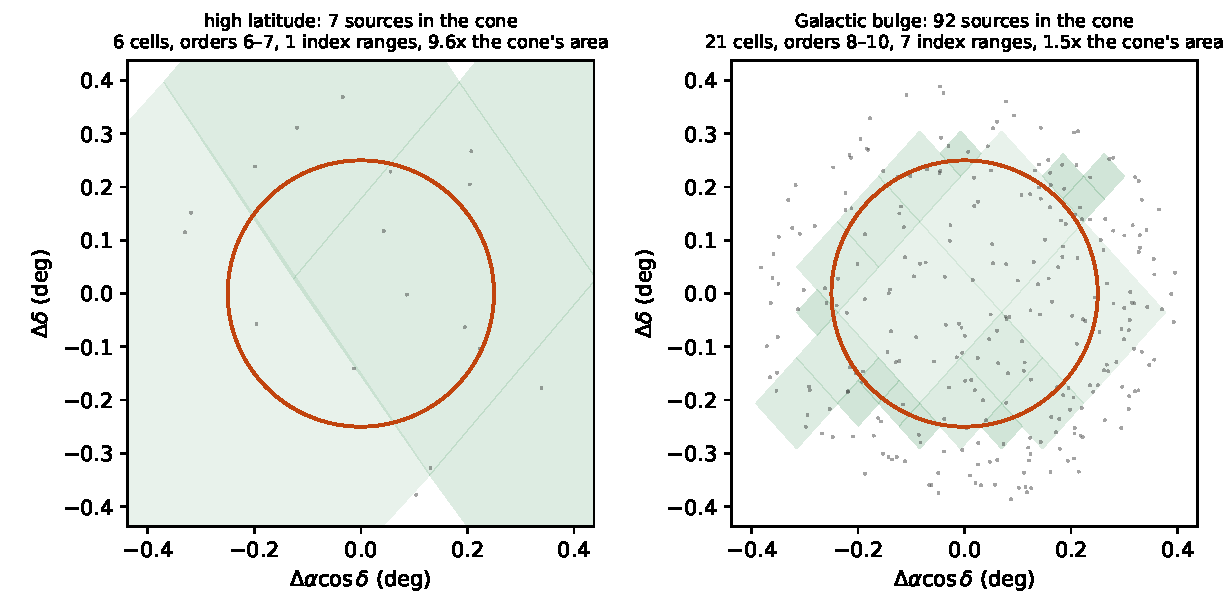
\includegraphics[width=\textwidth]{fig_covering.pdf}
  \caption{The same 0.25\degr\ cone covered in two places on the same catalogue.
    \emph{Left}: at high Galactic latitude the cost model buys one index range of
    large cells, covering 5.6 times the cone's area, because the 11 sources in the
    cone leave almost nothing to exclude. \emph{Right}: in the Galactic bulge the
    same cone holds 1183 sources, and the model cuts two orders deeper -- 23 cells
    in 8 ranges, 1.3 times the cone's area -- because there the false positives
    cost more than the ranges save. Grey dots are catalogue sources, the heavy
    circle the query cone, and the shaded quadrilaterals the covering cells, drawn
    from their own corners.}
  \label{fig:covering}
\end{figure*}

Figure~\ref{fig:covering} shows the two extremes on the same cone radius: at high
Galactic latitude the covering is a single range of large cells covering 5.6 times the
cone's area, because there is almost nothing to exclude; in the bulge the same cone is
covered by 23 cells in 8 ranges covering 1.3 times its area, because there the rows
removed are worth the extra ranges.

Two guards keep the model honest. A histogram is a coarse synopsis, and a dense cluster
split by the space-filling curve into pieces smaller than one bucket can be
underestimated; a partly covered cell is therefore never allowed to exceed a multiple
(64 by default) of the region's own area, which bounds the damage to the
density-proportional behaviour a fixed-depth covering would have had. Gaps between
ranges are merged when the rows they contain cost less than the range they save.

\subsection{Cells tested by their own geometry}

Whether a cell is inside, outside or on the boundary of the region has to be decided
conservatively -- a cell wrongly called outside loses rows -- but not crudely, because
every unnecessary cell is false positives at query time. Approximating each cell by a
cap of the largest pixel radius found anywhere on the sphere, the simplest safe choice,
is loose by a large factor for most cells.

\texttt{skycell} instead uses the cell's own four corners, computed from the continuous
HEALPix face coordinates, and the great-circle chords between them. A cell lies inside a
cone when its farthest corner does; it lies outside when the distance from the cone's
centre to every chord exceeds the radius. The chords are not the cell's edges, which
bow outwards, so each edge's departure from its chord is measured for that cell from
the edge midpoint. This matters at the poles, where an edge spans a large range of
azimuth and departs from its chord by a fraction of the cell's size rather than by its
square: a global constant fitted away from the poles produces false negatives there,
which is exactly what the validation of Sect.~\ref{sec:validation} caught during
development.

\subsection{Regions as stored objects}

A footprint is covered by a small number of cells written in the \texttt{NUNIQ}
encoding of the MOC standard and stored one per row in an ordinary B-tree. The
footprints containing a given position are those whose cell is one of that position's
ancestors, a short list of equality lookups; the exact geometry is then applied to the
candidates. Since a MOC's cells are disjoint by construction, no duplicate elimination
is needed. Refinement of these coverings stops when cells become negligible next to the
region, which keeps the ancestor list short: without that stop, boundary cells whose
siblings all fall outside keep splitting at no cost in cell count, and the lookup pays
for orders that carry almost no area.

\subsection{The query surface}

The extension exposes ADQL's own vocabulary: types \texttt{skypos} and
\texttt{skyregion} and functions \texttt{point}, \texttt{circle}, \texttt{box},
\texttt{polygon}, \texttt{contains}, \texttt{intersects}, \texttt{distance},
\texttt{area}, \texttt{coord1}, \texttt{coord2} and \texttt{centroid}, so that a
translator emits the standard's spelling rather than a dialect. The operator form
\texttt{pos <@ circle(\ldots)} is the one a planner can answer from an index; the
function form returns the same rows.

Beside the geometry, archives need the astrometry that decides \emph{where} a source
is at the epoch being asked about. \texttt{skycell} implements the IVOA UDF registry's
names -- \texttt{ivo\_epoch\_prop}, \texttt{ivo\_epoch\_prop\_pos},
\texttt{ivo\_apply\_pm}, \texttt{ivo\_healpix\_index}, \texttt{ivo\_healpix\_center} --
with the rigorous epoch propagation of the Hipparcos catalogue \citep{hipparcos}, in
which the star follows a straight line in space so that parallax, proper motion and
radial velocity all evolve together. Propagating a six-parameter solution forward and
back returns the starting position to better than a microarcsecond
(Sect.~\ref{sec:validation}). Frame conversions between ICRS, Galactic and ecliptic
coordinates are provided for the same reason.

An index built on catalogue positions cannot know where a star has moved to, so a
proper-motion-aware cone search is written as an indexable cone widened by the largest
motion of interest, intersected with an exact test on the propagated position.
Table~\ref{tab:ops} lists the surface.

\begin{table*}
  \caption{The query surface. ADQL spellings are used unchanged; the
    \texttt{skycell\_}-prefixed aliases exist for schemas where a name collides with
    one in \texttt{pg\_catalog}.}
  \label{tab:ops}
  \centering
  \small
  \begin{tabular}{l l}
    \hline\hline
    Signature & Meaning \\
    \hline
    \multicolumn{2}{l}{\emph{Geometry (ADQL)}}\\
    \texttt{point(frame, ra, dec)} & position $\rightarrow$ \texttt{skypos} \\
    \texttt{circle(frame, ra, dec, r)} & cone $\rightarrow$ \texttt{skyregion} \\
    \texttt{box(frame, ra, dec, w, h)} & box $\rightarrow$ \texttt{skyregion} \\
    \texttt{polygon(frame, ra, dec, ...)} & convex polygon \\
    \texttt{contains(a, b)}, \texttt{intersects(a, b)} & 1 or 0 \\
    \texttt{distance(a, b)}, \texttt{area(r)} & degrees, square degrees \\
    \texttt{coord1/coord2/centroid} & components, centre \\
    \texttt{pos <@ region} & indexable containment \\
    \hline
    \multicolumn{2}{l}{\emph{Astrometry (IVOA UDF registry)}}\\
    \texttt{ivo\_epoch\_prop(...)} & six parameters propagated \\
    \texttt{ivo\_epoch\_prop\_pos(...)} & position only \\
    \texttt{ivo\_apply\_pm(...)} & proper motion only \\
    \texttt{ivo\_healpix\_index/center} & cell of position, and back \\
    \texttt{icrs2gal}, \texttt{gal2icrs} & frame conversion \\
    \texttt{icrs2ecl}, \texttt{ecl2icrs} & frame conversion \\
    \hline
    \multicolumn{2}{l}{\emph{Index and covering}}\\
    \texttt{skycell\_ang2cell(ra, dec)} & the order-29 key \\
    \texttt{skycell\_cone/poly(cell, ...)} & indexable predicates \\
    \texttt{skycell\_cone\_ranges(...)} & ranges as rows (\texttt{LATERAL}) \\
    \texttt{skycell\_cone\_moc(...)} & covering as \texttt{NUNIQ} cells \\
    \texttt{skycell\_ancestors(cell, ...)} & a position's containing cells \\
    \hline
  \end{tabular}
\end{table*}

\section{Implementation}
\label{sec:impl}

The extension is written in C against the PostgreSQL 15+ server API and consists of a
geometry layer with no database dependencies -- HEALPix arithmetic, region predicates
and the covering -- and a layer that connects it to the planner.

The connection is a \emph{planner support function}
(\texttt{SupportRequestSimplify}), the mechanism PostGIS uses for
\texttt{ST\_DWithin}. Before path generation, a predicate such as
\texttt{point('ICRS', ra, dec) <@ circle('ICRS', $\alpha$, $\delta$, $r$)} is replaced by
a disjunction of range conditions on the key expression, conjoined with the exact test:

\begin{quote}\small\ttfamily
(cell BETWEEN lo1 AND hi1\\
 OR cell BETWEEN lo2 AND hi2 OR ...)\\
AND skycell\_in\_region(point(ra, dec),\\
\hspace*{6em}circle(...), 0.29)
\end{quote}

The key expression is not written by the user: the support function builds the
candidate expression from the predicate's position argument and keeps it only if the
relation actually carries an index on it, so the same query text works whether
positions are stored as two columns or as a \texttt{skypos} column. Because the index
conditions are then ordinary range predicates, the planner estimates their selectivity
from the same histogram, and the last argument of the exact test carries the fraction
of the covering that the region occupies, so that the product of the two estimates is
close to the truth. This is why the row estimates in Sect.~\ref{sec:results} are
accurate, and accurate estimates are what keep a spatial predicate from being joined in
the wrong order in a larger query.

Two caches matter for planning cost. The density model and the identity of the matching
index are cached per backend and dropped whenever statistics, the relation or the
relation cache change; coverings are memoised by region and statistics source, since a
service plans the same cone many times. Measured on a real corpus, the first cache is
worth 45--70\,\textmu s per plan and the second up to 50\,\textmu s for the larger
regions.

For joins, where the region is not a constant, the rewrite emits a fixed number of
range slots computed per outer row -- the structure \texttt{q3c\_join} uses -- while a
set-returning function \texttt{skycell\_cone\_ranges()} offers the alternative of a
variable number of ranges through a \texttt{LATERAL} join. The two differ in plan shape
rather than geometry, and Sect.~\ref{sec:results} shows the difference is large.

\section{Validation}
\label{sec:validation}

A covering that misses a cell silently loses rows, so correctness is established by
brute force rather than by inspection, at three levels.

The HEALPix layer is checked against known cell centres, round trips between positions
and cells at all 30 orders, the nesting property, equal area, and the bound the covering
relies on -- that no point of a cell lies farther from its centre than its farthest
corner -- over 1.6 million sampled points including the poles, the boundary between the
polar and equatorial zones, and the base-pixel edges.

The covering is checked against a 2-million-point clustered catalogue for cones from
1\arcsec\ to 120\degr\ and for convex polygons, and against 30\,000 adversarial cones
-- at the poles, across the zone boundary, at $\alpha = 0$ and on face edges, with radii
from 0.02\,mas to 10\degr\ -- with 200 points sampled inside each, half of them within
a part per billion of the rim. Both assert zero false negatives. This is the test that
caught the polar edge-bulge error of Sect.~\ref{sec:method}.

At the SQL level, two regression suites require that every indexed answer equals the
answer from a sequential scan with the exact predicate: 240 cones in two configurations,
60 polygons, both join forms and the MOC footprint lookup in the first; the ADQL
surface, the operator and function spellings over 120 random regions, the presence of
index plans (and their absence when the region is not constant), epoch-propagation
round trips and frame conversions in the second.

\section{Benchmark}
\label{sec:bench}

\subsection{Corpus}

The catalogue is 10 million synthetic sources with a density contrast resembling a real
optical survey: 35\% uniform on the sphere, 45\% in a Galactic disk (longitude uniform,
latitude exponential with a 3\degr\ scale), 12\% in a bulge (Gaussian, 7\degr), and 8\%
in 200 clusters with dispersions from 0.02\degr\ to 0.5\degr. Positions are drawn
deterministically from a seed. Peak densities exceed the mean by more than three orders
of magnitude, which is what makes the density model's job non-trivial.

\subsection{Targets}

Q3C 2.0.5, pgSphere 1.5.2 and \texttt{skycell} each hold the same logical rows in their
own natural layout: Q3C an expression B-tree on \texttt{q3c\_ang2ipix} with the table
sorted along the same curve; pgSphere an \texttt{spoint} column with a GiST index;
\texttt{skycell} a \texttt{bigint} cell column with a B-tree and a 1000-bucket
histogram. All three tables are physically ordered along a space-filling curve, so heap
locality is held equal. Queries are the documented interface of each extension:
\texttt{q3c\_radial\_query}, \texttt{spoint <@ scircle} and \texttt{skycell\_cone}.

\subsection{Protocol}

Each measurement is a fixed set of query centres, half drawn from catalogue positions
(hence density-weighted) and half uniform on the sky, run once to warm and once to
measure, with a third pass under \texttt{EXPLAIN (ANALYZE, BUFFERS)} to record buffers,
planning time and the planner's row estimate against the actual count. Cone radii span
1\arcsec\ to 3\degr\ with 16--400 queries each. Cross-matches join a 200\,000-row probe
table -- half catalogue sources displaced by $\sim$0.3\arcsec, half uniform -- to the
catalogue. Footprint queries ask which of 20\,000 stored circles contain each of the
200\,000 probes. All row counts are compared between methods.

Everything runs on one machine: PostgreSQL 18.6 in a Docker Desktop virtual machine on
an 11-core Apple Silicon laptop, 8\,GB of memory, \texttt{shared\_buffers} 2\,GB, JIT
off and parallel query disabled so that each measurement is one core doing one query.
Absolute numbers are therefore properties of this machine; the comparisons are between
methods measured on it within minutes of each other.

Two biases are worth naming. The corpus is synthetic and its density structure was
chosen by the author of the method under test. And the three methods are measured in
separate phases, so a phase measured later benefits from a warmer cache; the control in
Sect.~\ref{sec:interleaved} quantifies that.

\section{Results}
\label{sec:results}

All three methods return identical row counts on every query of the grid. In the
cross-matches pgSphere returns one or two more pairs out of $\sim$100\,000, consistent
with its $10^{-9}$\,rad comparison tolerance counting sources exactly on the rim.

\subsection{Cone searches}

\begin{table*}
  \caption{Cone searches on the 10-million-source catalogue: median query time
    (planning and execution), buffer pages touched, and the error of the planner's
    row estimate (median of $\max(\mathrm{est}/\mathrm{act}, \mathrm{act}/\mathrm{est})$).
    All three methods return identical row counts on every query.}
  \label{tab:cones}
  \centering
  \begin{tabular}{l r r r r r r r r r r}
    \hline\hline
    & & \multicolumn{3}{c}{median time (ms)} & \multicolumn{3}{c}{buffers} & \multicolumn{3}{c}{estimate error} \\
    \cline{3-5}\cline{6-8}\cline{9-11}
    radius & $\langle$rows$\rangle$ & Q3C & pgSphere & skycell & Q3C & pgSphere & skycell & Q3C & pgSphere & skycell \\
    \hline
    1\arcsec   &      0.5 & 1.330 & 0.035 & \textbf{0.024} & 301 &   5.8 & \textbf{3.9}  & 1.00 & 1.00 & 1.00 \\
    10\arcsec  &      0.7 & 1.374 & 0.030 & \textbf{0.023} & 301 &   5.6 & \textbf{4.3}  & 1.00 & 1.00 & 1.00 \\
    1\arcmin   &      3.4 & 1.366 & 0.032 & \textbf{0.024} & 301 &   6.4 & \textbf{5.3}  & 1.00 & 1.00 & 1.00 \\
    6\arcmin   &     80.1 & 1.353 & 0.038 & \textbf{0.033} & 303 &  13.6 & \textbf{9.3}  & 2.00 & 4.00 & \textbf{1.46} \\
    30\arcmin  &      516 & 1.373 & 0.095 & \textbf{0.075} & 313 &  61.4 & \textbf{30.1} & 1.92 & 2.92 & \textbf{1.16} \\
    1\degr     &    1\,476 & 1.427 & 0.315 & \textbf{0.139} & 329 &   154 & \textbf{55.5} & 1.89 & 2.78 & \textbf{1.22} \\
    3\degr     &   20\,652 & 3.023 & 1.010 & \textbf{0.573} & 649 &   617 & \textbf{343}  & 2.32 & 2.93 & \textbf{1.10} \\
    \hline
  \end{tabular}
\end{table*}

\begin{figure*}
  \centering
  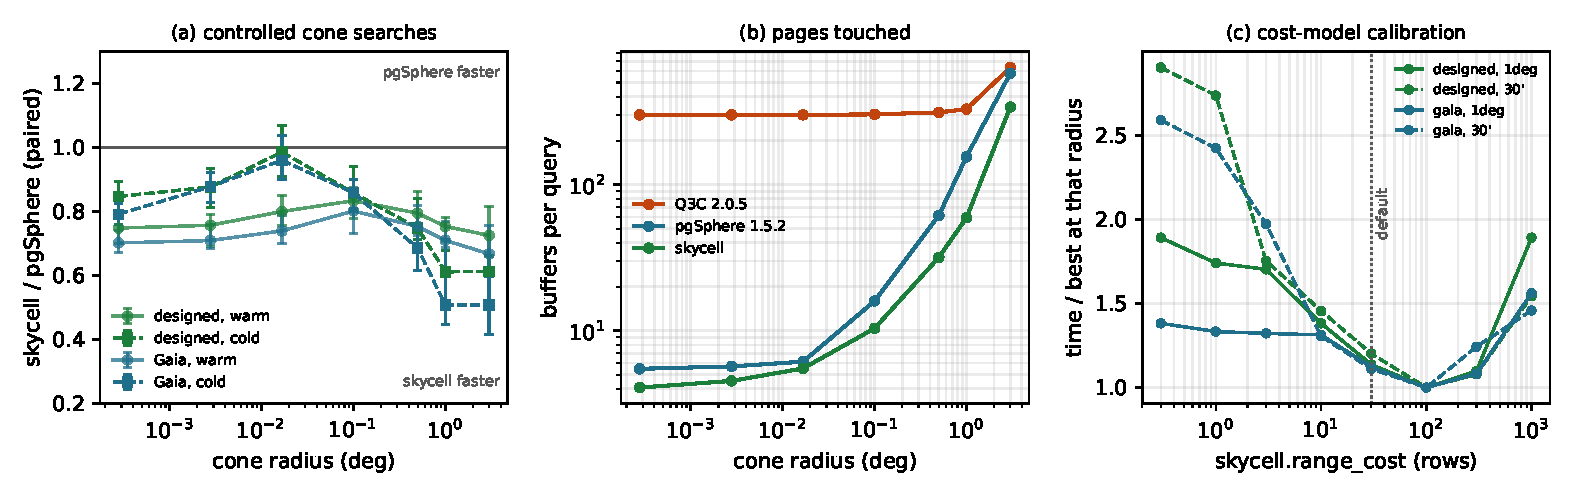
\includegraphics[width=\textwidth]{fig_benchmark.pdf}
  \caption{Cone searches and cross-matching on the 10-million-source catalogue.
    \emph{(a)} median query time against cone radius, planning included;
    \emph{(b)} buffer pages touched per query; \emph{(c)} wall time of a
    200\,000-probe cross-match at 1\arcsec\ and 10\arcsec, with the two plan shapes
    \texttt{skycell} offers for the same geometry. Note the logarithmic axes in
    (a) and (b).}
  \label{fig:benchmark}
\end{figure*}

Table~\ref{tab:cones} and Fig.~\ref{fig:benchmark}a give the medians. \texttt{skycell}
is fastest at every radius, by a factor 1.3--1.5 against pgSphere below 6\arcmin\ and
2.3 at 1\degr. Q3C is an order of magnitude slower on small cones for a structural
reason: version 2.0.5 expands \emph{every} \texttt{q3c\_radial\_query} into 100 key
ranges regardless of radius, which costs about 300 buffer pages and 1.2\,ms of planning
before any row is read. Its cross-match path, which uses four ranges per probe, does not
pay this.

The buffer counts (Fig.~\ref{fig:benchmark}b) show where the difference comes from at
large radii: at 1\degr\ \texttt{skycell} touches 55 pages against pgSphere's 154, and at
3\degr\ 343 against 617, because a covering sized by the cost model wastes less area
than a tree of bounding boxes whose leaves were built without reference to the query.

\subsection{Polygons, cross-matches and footprints}

Convex polygons of 0.05\degr--2\degr\ take a median 0.142\,ms against pgSphere's
0.631\,ms and Q3C's 1.526\,ms; pgSphere's mean (3.9\,ms) and 95th percentile (20\,ms)
are far above its median, which the per-query records trace to polygons whose bounding
volume is a poor fit.

Cross-matching 200\,000 probes at 1\arcsec\ takes 0.47\,s with the \texttt{LATERAL}
form, against 1.12\,s for \texttt{skycell}'s own join form, 1.95\,s for
\texttt{q3c\_join} and 2.85\,s for pgSphere (Fig.~\ref{fig:benchmark}c). The gap
between the two \texttt{skycell} forms is plan shape, not geometry: the join form and
\texttt{q3c\_join} both build a bitmap from several bitmap index scans for every probe,
while the \texttt{LATERAL} form issues plain range scans, as many as that probe's
covering needs. With a covering index the same query becomes an index-only scan and
0.59\,s at 10\arcsec.

For stored footprints, the MOC-in-a-B-tree arrangement answers 140\,996 point-in-region
pairs in 0.67\,s against pgSphere's 1.10\,s, at the cost of an index that is larger
(10\,MB against 1.2\,MB) and slower to build (1.1\,s against 0.04\,s), since a region
becomes several rows rather than one.

\subsection{Index size, build time and estimates}

\begin{table}
  \caption{Storage and build cost for the same 10 million sources. Table sizes
    differ because each method stores its own position representation alongside the
    catalogue columns. \texttt{ANALYZE} is slower for \texttt{skycell} because the
    histogram is computed over an expression.}
  \label{tab:build}
  \centering
  \begin{tabular}{l r r r r}
    \hline\hline
    method & table & index & build & \texttt{ANALYZE} \\
           & (MB)  & (MB)  & (s)   & (s) \\
    \hline
    Q3C      & 574 & 214 &  1.8 & 0.16 \\
    pgSphere & 730 & 683 & 43.9 & 0.85 \\
    skycell  & 652 & 214 &  2.3 & 1.40 \\
    \hline
  \end{tabular}
\end{table}

The B-tree of 64-bit keys is 214\,MB and builds in 2.3\,s; pgSphere's GiST is 683\,MB
and builds in 44\,s (Table~\ref{tab:build}). For an archive this is an operational
number: it is what an ingest, a restore or a schema migration has to pay.

The planner's row estimate for a 1\degr\ cone is off by a median factor 1.22 for
\texttt{skycell}, against 1.89 for Q3C and 2.78 for pgSphere, because the rewritten
predicate is a range condition on an ordinary expression and the planner estimates it
from the ordinary histogram.

\subsection{Ablations}

Switching off the density model, removing the area guard, or moving $c_{\rm range}$
between 3 and 30 changes small-cone times by a few percent on this catalogue: with cells
much larger than the cone, the covering is one or two cells whatever the model says.
The density model earns its place on medium cones in crowded fields, which is where
Fig.~\ref{fig:covering} shows it cutting finer, and on the false positives that would
otherwise be read.

\subsection{An interleaved control}
\label{sec:interleaved}

Because the grid measures methods in separate phases, we repeated the cone searches
alternating the two methods query by query, warm, with \texttt{skycell} going first --
the order that disadvantages it. The ratios of \texttt{skycell} to pgSphere are then
0.85, 1.04, 0.92, 0.72 and 0.61 at 1\arcsec, 1\arcmin, 30\arcmin, 1\degr\ and 3\degr:
the advantage survives at every radius but one, where the two tie, with smaller margins
than the phase-ordered grid. The grid should be read as the optimistic end of the range
and this control as the conservative one.

\section{Inside a TAP service}
\label{sec:tap}

A benchmark of index operations is not a benchmark of an archive. We therefore ran the
same build inside \texttt{egernia} \citep{egernia}, a TAP 1.1 server, against its
published 500\,096-row ObsCore corpus, in an A/B where one database held both indexes
and two otherwise identical service processes differed only in how they translate
\texttt{CONTAINS}: one to pgSphere, one to \texttt{skycell}. The service's own harness
interleaved the two targets rung by rung.

Both targets pass the conformance gate (\texttt{taplint}, zero errors) and the
cross-server agreement gate on all eleven portable query classes, and the 203 cone
queries of the corpus return identical rows through both translations.

The performance result is a tie: all 18 comparison cells, across the mixed workload and
five query classes at 1, 8 and 32 clients, fall inside the protocol's tie rule, with
throughput ratios between 0.96 and 1.06. At the database level \texttt{skycell} is
1.2--1.45 times \emph{slower} per query than pgSphere on that corpus.

Both facts have the same cause. A cone query over half a million rows returns tens to
hundreds of rows and costs a fraction of a millisecond either way, against roughly
10\,ms of CPU per request spent in the service's own Python; and at that relation size
there is no scan left for a better covering to shorten, while the covering still has to
be planned. The measurements put the crossover at a few million rows.

\section{Discussion}

The results support a narrow claim: on large catalogues, a covering sized by cost over
an equal-area integer key is faster than both established extensions for the operations
measured, with a smaller index and better row estimates, and it does not give up the
ability to index regions. They do not support the claim that it is the better choice
everywhere. On a small, already well-clustered relation it is slower, and inside a
service whose cost is dominated by protocol handling it changes nothing at all.

What remains expensive is planning. A covering is computed per plan, and even cached it
costs 0.01--0.12\,ms, against 0.006\,ms for a GiST predicate that needs no such step.
The architectural way out is to stop planning ranges: an SP-GiST operator class over the
cell hierarchy would present a single index qualification to the planner and refine
during the index descent, where the work is proportional to the rows actually present
rather than to the region. That would also remove the per-arm cost the planner pays for
a disjunction of ranges, which our measurements put at 15--20\,\textmu s each.

The density synopsis is the other limit. An equi-depth histogram over a space-filling
curve is a poor two-dimensional density estimator: a cluster split by the curve into
pieces smaller than one bucket is invisible to it, which is why the area guard exists.
A custom \texttt{typanalyze} storing a multi-order density map -- a MOC with counts --
would estimate what the covering actually needs, and would also improve selectivity
estimates for crowded fields.

Finally, nothing here has run on real data at Gaia density, with cold caches, or on
more than one machine, and the corpus was designed by the same author as the method.

\section{Conclusions}

\texttt{skycell} keeps Q3C's compact integer key and B-tree while answering the region
queries pgSphere was built for, by treating the depth of a covering as a cost question
whose answer follows from the local source density and the price of an index range. On
a 10-million-source catalogue it is the fastest of the three for cone searches at every
radius tested, four times faster than pgSphere for convex polygons, four times faster
than Q3C for cross-matching, faster for point-in-footprint queries, and it keeps an
index a third the size of pgSphere's with row estimates twice as accurate. An
interleaved control puts the cone-search advantage at 0.61--1.04 times pgSphere's time
rather than the larger factors of the phase-ordered grid.

The same build is slower on a 500\,000-row table and makes no difference to a TAP
server's published throughput, because there the database is a small part of a request.
An index is worth choosing carefully when the scan dominates; the measurements here put
that crossover at a few million rows, which is where survey archives already are.

\section*{Data availability}

The extension, its test suites, the benchmark harness and the raw results of every
measurement quoted here are available at
\url{https://github.com/jesusjuansalgado/skycell} under the MIT licence. The
catalogue is generated from a seed by \texttt{bench/01\_data.sql}, so the corpus is
reproducible without transferring data; \texttt{bench/run.sh} reproduces
Tables~\ref{tab:cones} and~\ref{tab:build} and Figs.~\ref{fig:covering}
and~\ref{fig:benchmark} end to end. The TAP A/B of Sect.~\ref{sec:tap} is recorded,
protocol and results, in the same repository.

\begin{acknowledgements}
  The implementation, the benchmark harness and the analysis presented here were
  developed with the assistance of Anthropic's Claude Code. All measurements were
  produced by the software cited in the data availability section and can be
  reproduced from it.
\end{acknowledgements}
